\chapter{Methods}\label{chap:methods}
Before jumping to our main task we want to point out some changes that we brought to the repository. The main purpose of these changes was to prevent more reworking in the future.
The below list shows the changes:
\begin{itemize}
    \item Split the repository codes to different .txt files.
    \item Adding \#endfile to all repository codes, will help us during tokenization. 
 Figure \ref{fig:sepRepo} shows the changes.
    \item Code restructure. Figure \ref{fig:restructure} shows the new repository structure.
\end{itemize}

\begin{figure}[H]
    \centering
    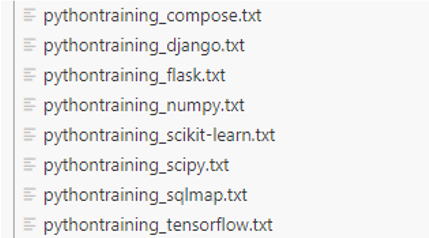
\includegraphics[width=0.5\linewidth]{spirate-repos.png}
    \caption{FinaltextX Array Element Error}
    \label{fig:sepRepo}
\end{figure}

\begin{figure}[H]
    \centering
    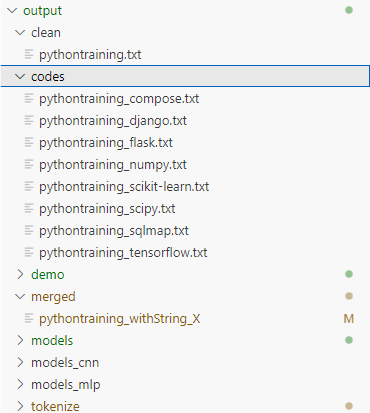
\includegraphics[width=0.5\linewidth]{restructure.png}
    \caption{FinaltextX Array Element Error}
    \label{fig:restructure}
\end{figure}

\section{Demo Presentation}
\subsection{First Step}
In the first step, we are required to run the \textit{trymodel.py} script. 
Running the mentioned script has some challenges due to code deprecation and structural changes brought before. 
The challenges that we faced are listed below:
\begin{itemize}
    \item \textbf{FinaltextX} conversion to arra, the reason behind this error was due to setting an array element with a sequence. The figure \ref{fig:array_error} shows the error. The solution for this issue was to create a method to convert an array that is compatible with a numpy array. Figure \ref{fig:array_changes} shows the solution with the changes.
    \item \textbf{yhat\_classes} variable had issue with shaping after adding pad sequence to \textit{X\_finaltest}, figure \ref{fig:error_dimentionality} shows the error. 
 The solutions for the mentioned issue are listed below:
        \begin{enumerate}
            \item Multipying \textit{max\_lenght} by 300 because the vector lenght was changed in \textit{convert\_to\_array} method which Figure \ref{fig:max_lenght_muliplication} shows the solution.
            \item Change the \textbf{yhat\_classes} variable value to \textit{predict} and take it back with the help of numpy \textit{argmx} method. The changes are shown in figure \ref{fig:yhat_changes}.
            \item Adding \textit{zero\_devision = 1} and \textit{average=\'macro\'} to the precision. Figure \ref{fig:precision_changes} shows the changes.
            \item Adding \textit{average=\'macro\'} to \textit{recall} and \textit{F1Score} varaibles. Figure \ref{fig:precision_changes} shows the changes.
        \end{enumerate} 
\end{itemize}

\begin{figure}[H]
    \centering
    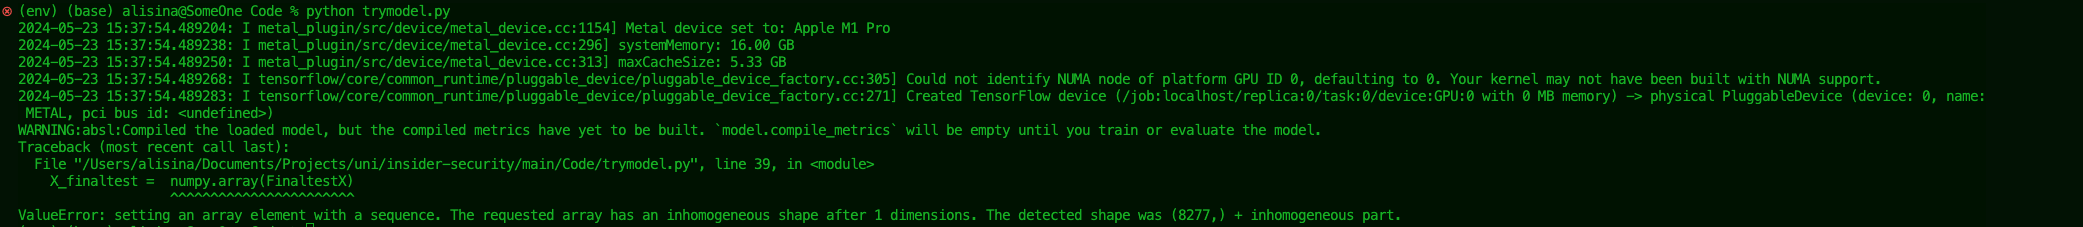
\includegraphics[width=1\linewidth]{array_error.png}
    \caption{FinaltextX Array Element Error}
    \label{fig:array_error}
\end{figure}

\begin{figure}[H]
    \centering
    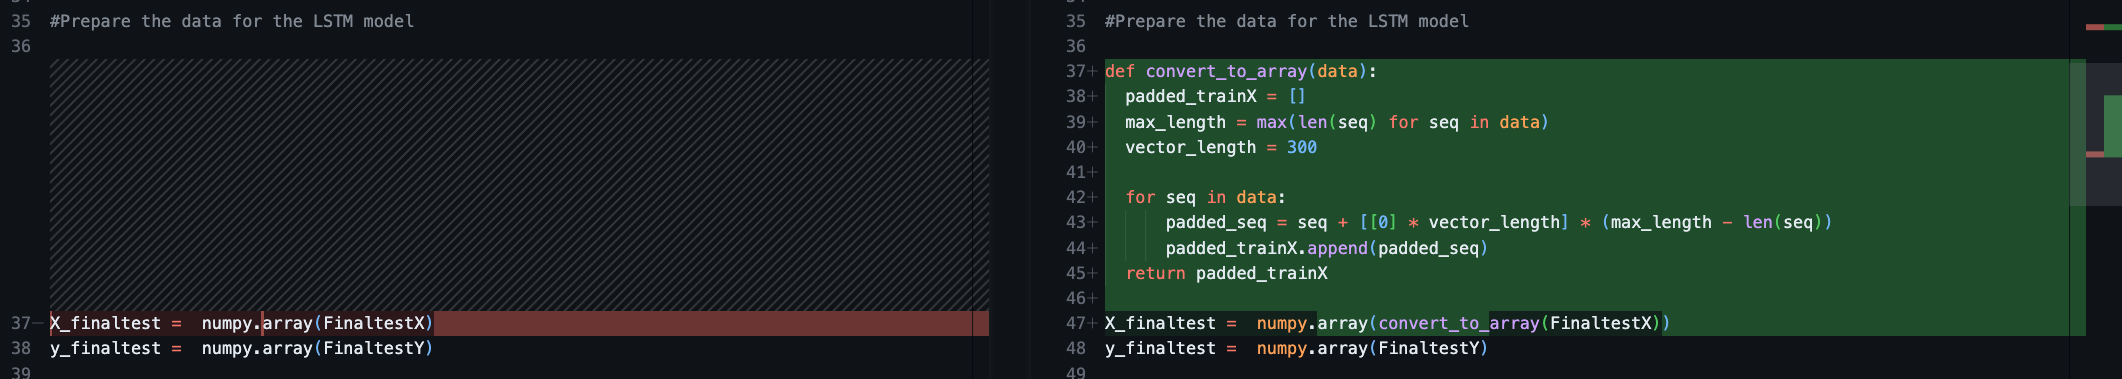
\includegraphics[width=1\linewidth]{array_changes.png}
    \caption{Implementation of convert to array method}
    \label{fig:array_changes}
\end{figure}

\begin{figure}[H]
    \centering
    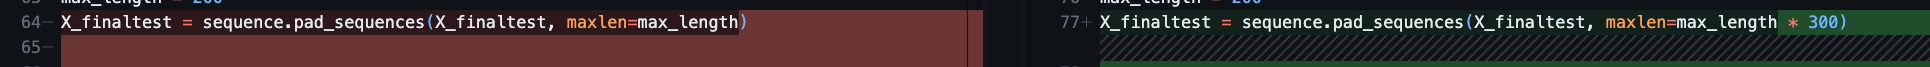
\includegraphics[width=1\linewidth]{X_finaltext_add_300.png}
    \caption{Predict issue}
    \label{fig:error_dimentionality}
\end{figure}

\begin{figure}[H]
    \centering
    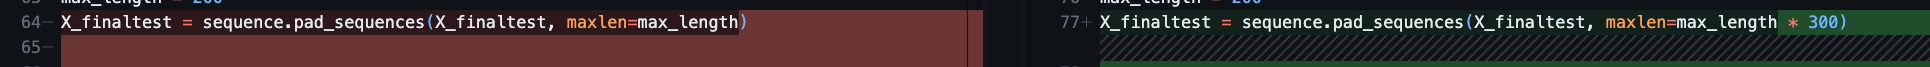
\includegraphics[width=1\linewidth]{X_finaltext_add_300.png}
    \caption{Max Lenght multiplication with 300}
    \label{fig:max_lenght_muliplication}
\end{figure}

\begin{figure}[H]
    \centering
    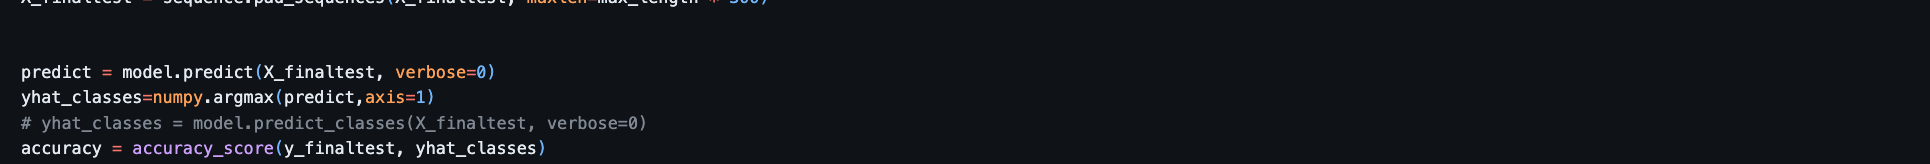
\includegraphics[width=1\linewidth]{changes yhat classes.png}
    \caption{Change on Yhat classes}
    \label{fig:yhat_changes}
\end{figure}

\begin{figure}[H]
    \centering
    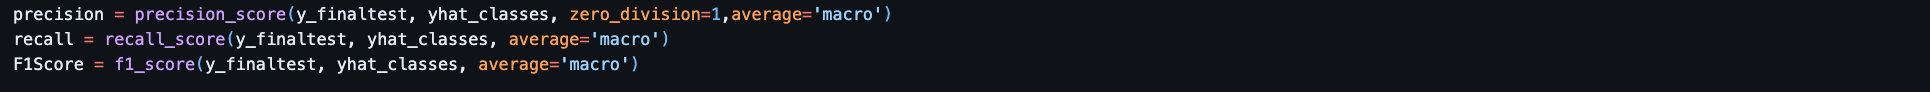
\includegraphics[width=1\linewidth]{precision_changes.png}
    \caption{Changes on Precision, Recall, F1Score variables}
    \label{fig:precision_changes}
\end{figure}


\section{Model Demonstration}
To demonstrate the model, we have to run the \textit{demonstrat.py} script. While running the mentioned script we have faced with issues in call \textit{myutils.getblocksVisual} method.
\begin{itemize}
    \item \textit{word\_vectors} vocab parameter deprication. Figure \ref{fig:W2V_issue} shows the error.
    \item \textit{W2v\_model} list is required to receive from \textbf{wv} parameter. Figure \ref{fig:W2V_issue} shows the error.
    \item While rendering the demonstrated image the text was layer over layer. In addition, it returned some errors related to text size. 
 Figure \ref{fig:issue_image_layer} shows the problem of the demonstrated image.
\end{itemize} 
The solution for this issue was to bring changes in the \textit{getblocksVisual} method. 
The changes are listed in the following:
 \begin{itemize}
    \item The vocab variable of \textit{word\_vectors} changed to \textit{key\_to\_index}.
    \item Deu to changes in \textit{W2v\_model} library, we need to use \textbf{wv} object to get array instead of directly receive it from \textit{W2v\_model}.
    \item Deu to changes in PIL library for python version 3.11 \textit{textsize} has an issue, so instead we used textbbox to handle the situation.
 Figure \ref{fig:text_size_prob_code} shows the original code of the repository and figure \ref{fig:text_size_updated} shows the code which was updated by us.
 The updated code uses \textit{d.textbbox} instead of \textit{d.textsize}. 
 The textbbox method provides a more accurate bounding box for the text, which is particularly useful for correctly calculating the width and ensuring precise placement of subsequent text. 
 The [2] index accesses the width from the bounding box tuple (left, top, right, bottom).
 The updates ensure that both the x and y positions are incremented consistently, which helps maintain the correct layout and spacing of the text within the image.
 \end{itemize}

 After fixing all the above issues we managed to successfully run the \textit{demonstrate.py} script. 
 Figure \ref{fig:succees_demonstrate} shows a successful log of run \textit{demonstrate.py} script.

 \begin{figure}[H]
    \centering
    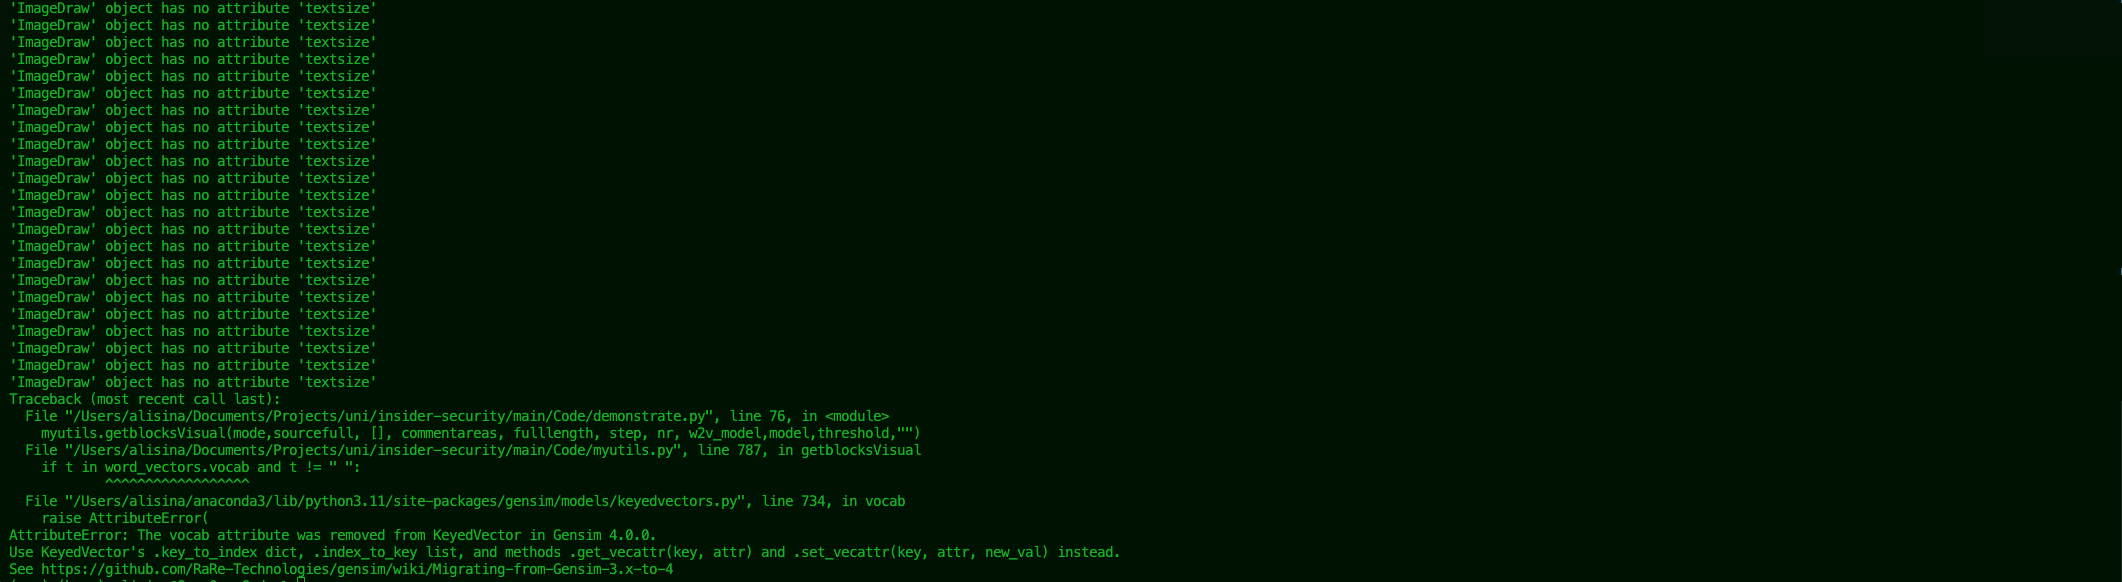
\includegraphics[width=1\linewidth]{w2v_issue.png}
    \caption{W2V code deprecation issues}
    \label{fig:W2V_issue}
\end{figure}
\begin{figure}[H]
    \centering
    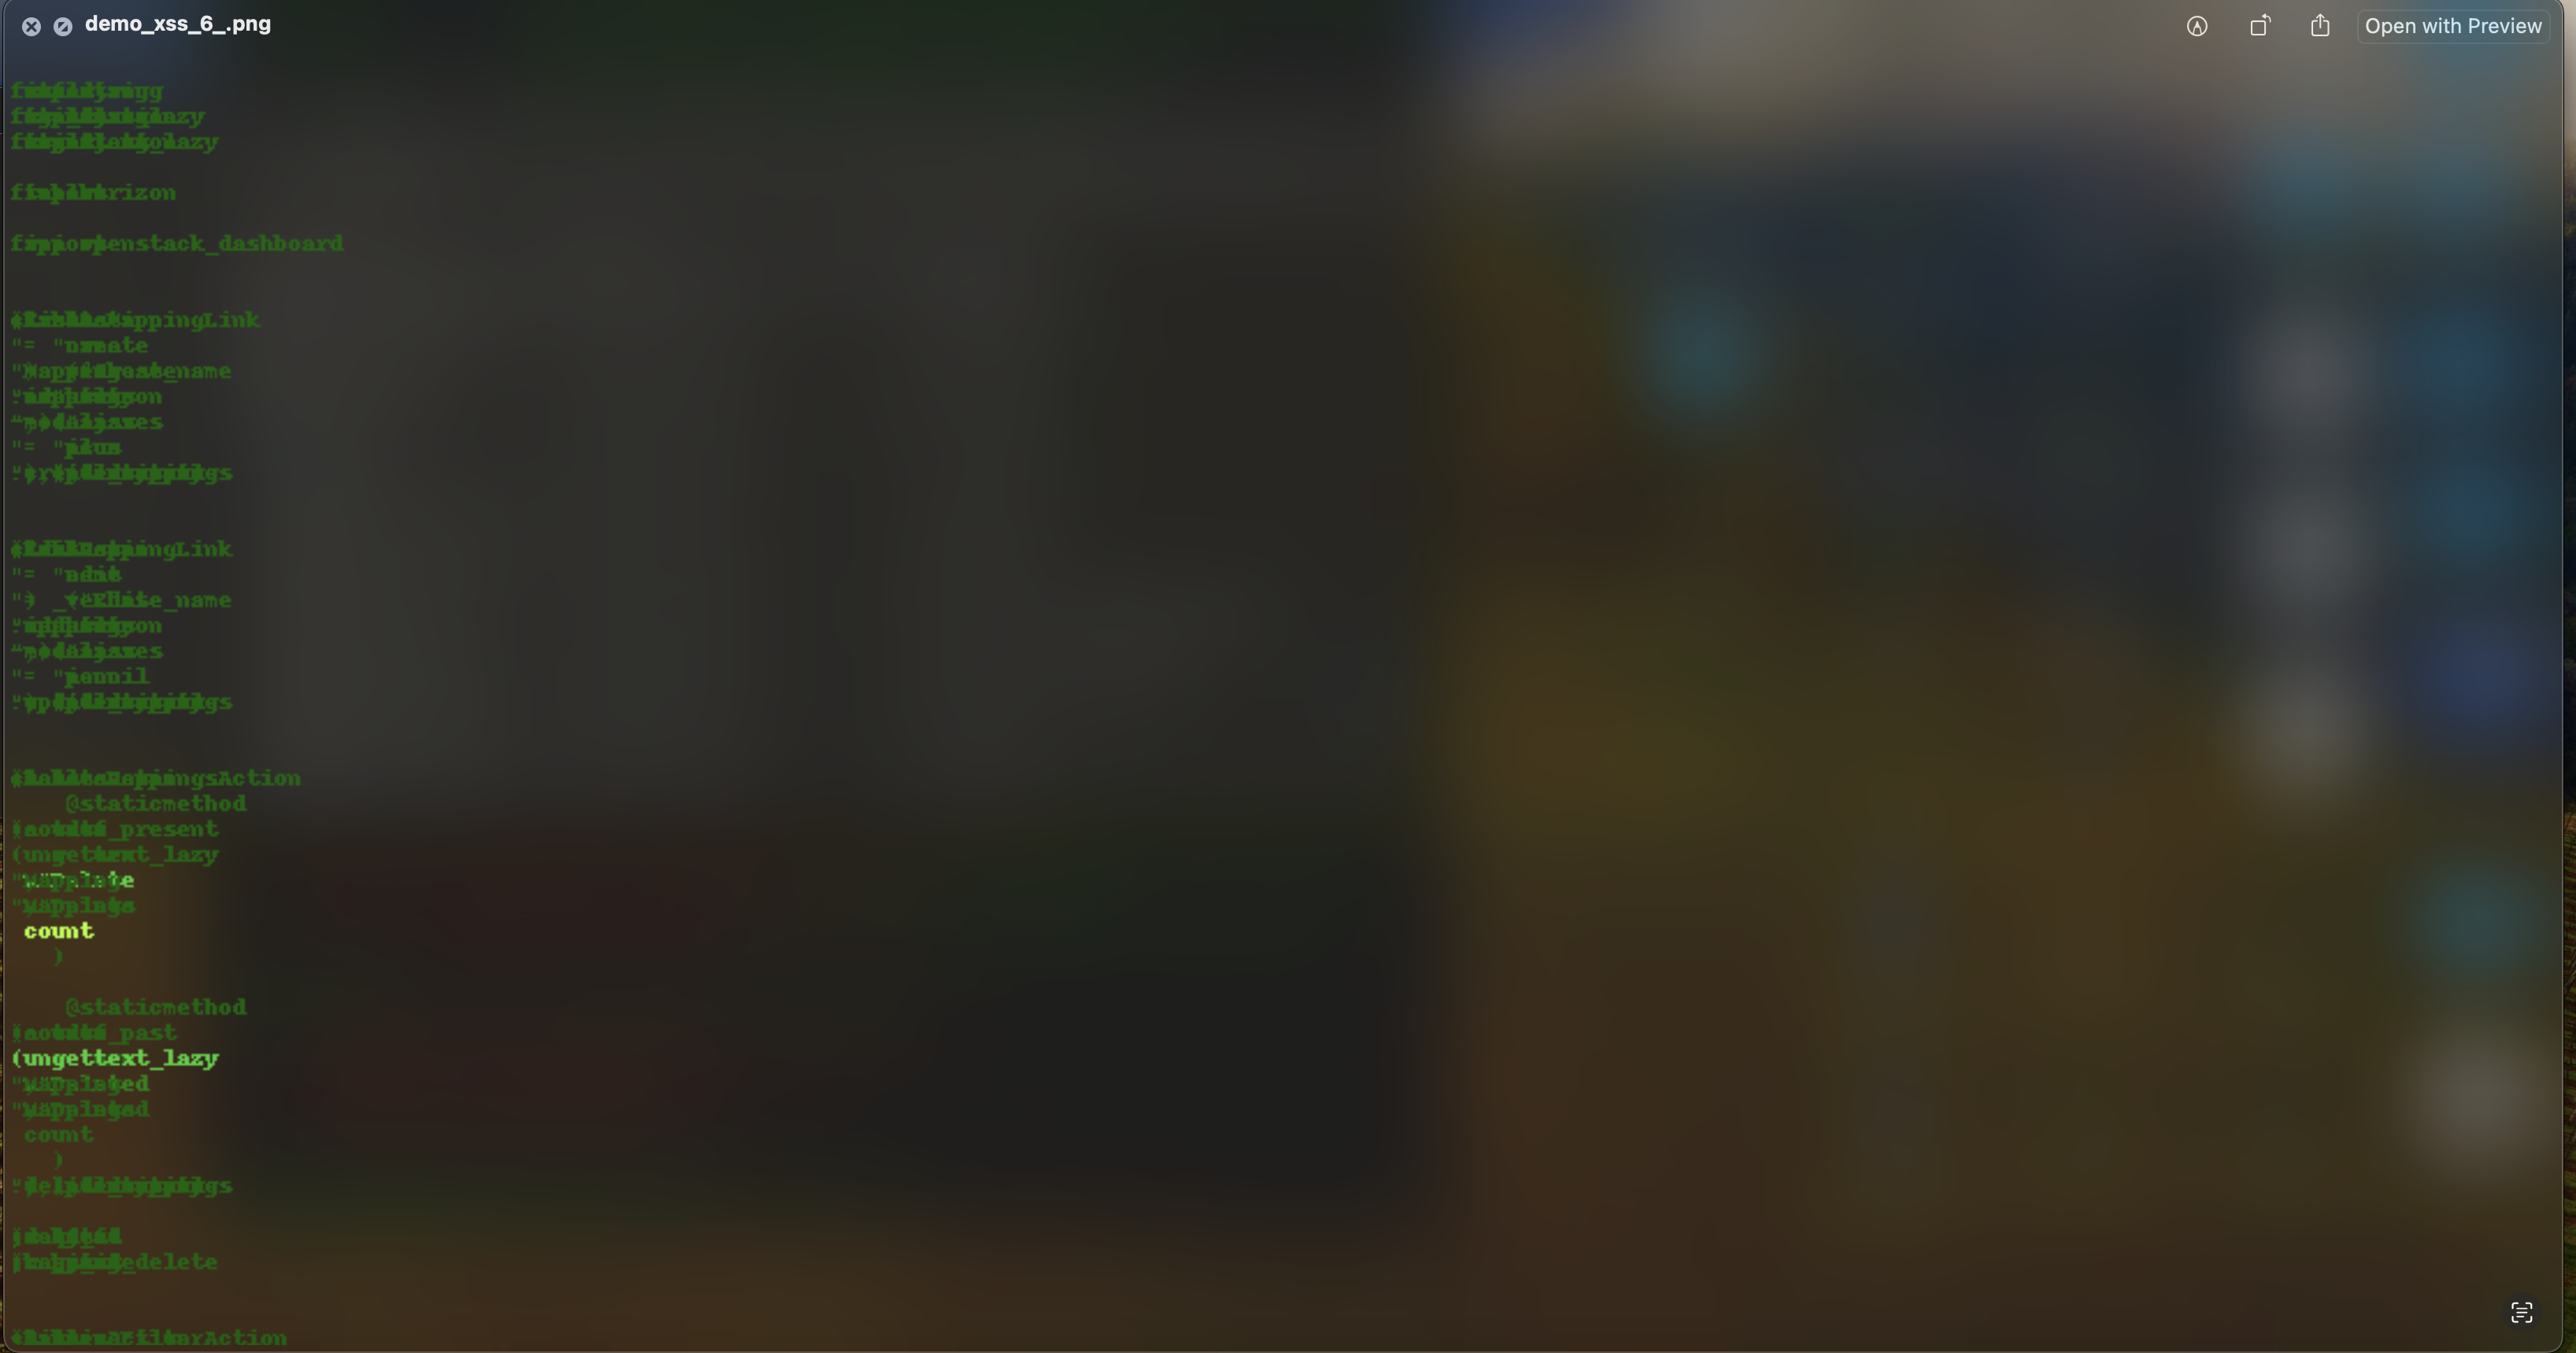
\includegraphics[width=1\linewidth]{issue_image_layer.png}
    \caption{Text layers issue in generated image}
    \label{fig:issue_image_layer}
\end{figure}

\begin{figure}[H]
    \centering
    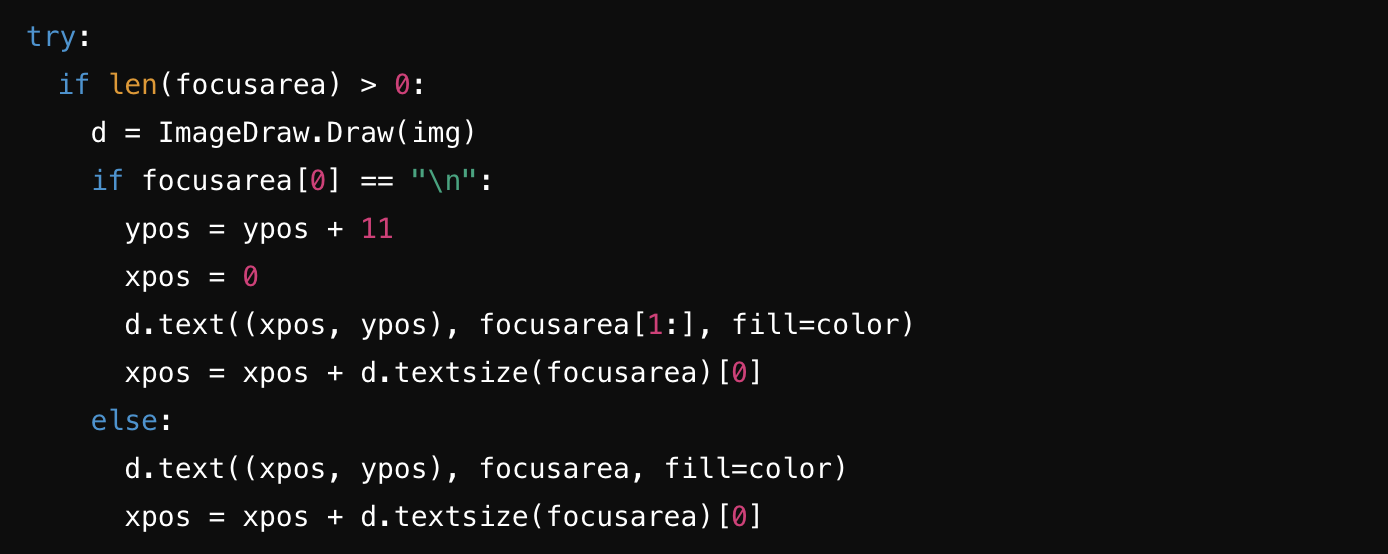
\includegraphics[width=1\linewidth]{text_size_code_1.png}
    \caption{Textsize original implemented code}
    \label{fig:text_size_prob_code}
\end{figure}
\begin{figure}[H]
    \centering
    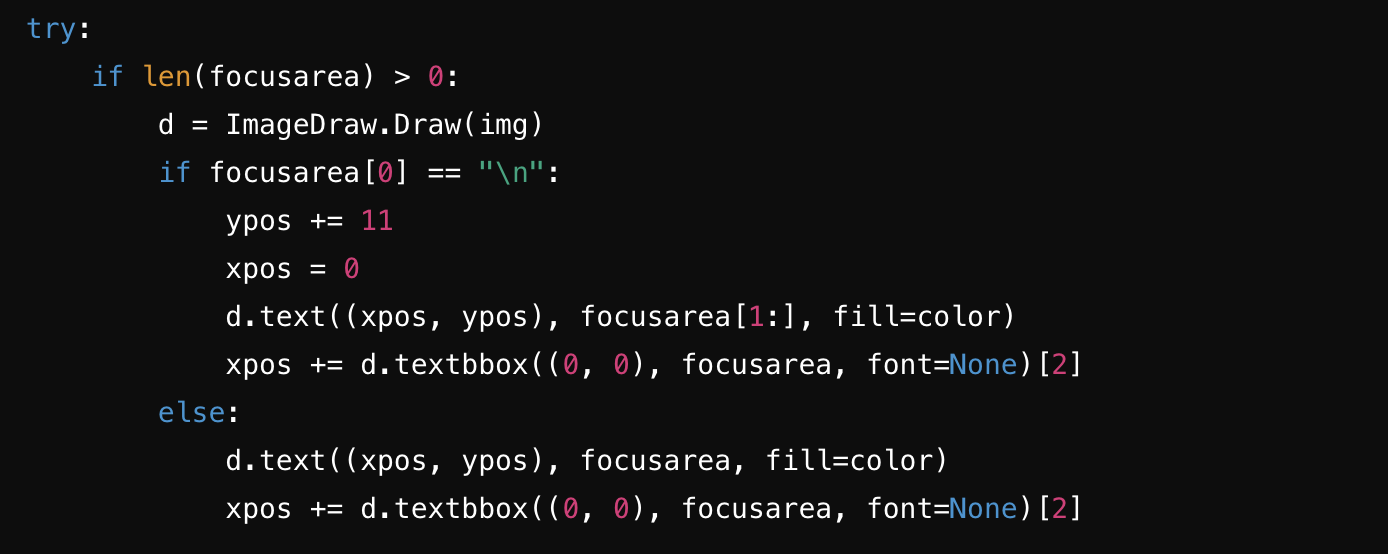
\includegraphics[width=1\linewidth]{text_size_updated.png}
    \caption{Text size updated code}
    \label{fig:text_size_updated}
\end{figure}

\begin{figure}[H]
    \centering
    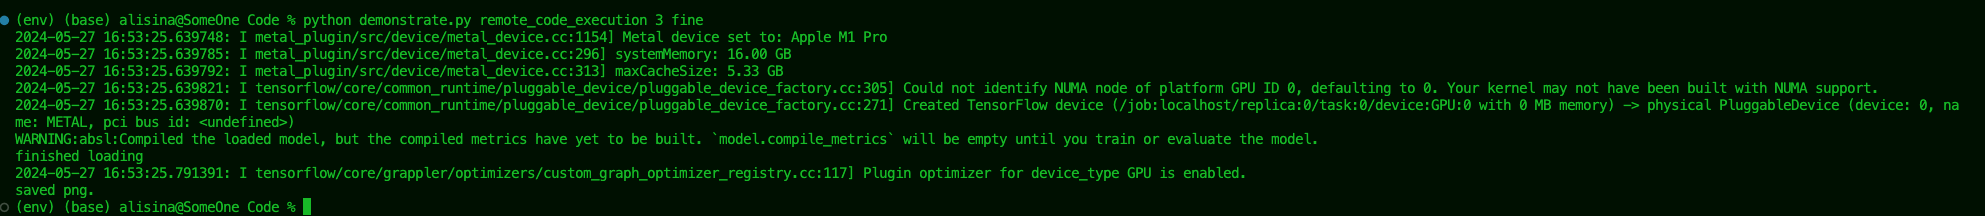
\includegraphics[width=1\linewidth]{success_demonstrate.png}
    \caption{Successfull running demonstrate script}
    \label{fig:succees_demonstrate}
\end{figure}


\section{Other ML Models}
\subsection{CNN}
To implement the CNN model we made the below changes:
\begin{itemize}
    \item We removed (\textit{from keras.preprocessing import sequence}) and add (\textit{from tensorflow.keras.preprocessing.sequence import pad\_sequences}).
    \item We add new lines such as:
        \begin{itemize}
            \item \textit{from tensorflow.keras.layers import Conv1D, MaxPooling1D, Flatten, Dense}
            \item \textit{from tensorflow.keras.utils import to\_categorical}
            \item \textit{model.add(Conv1D(64, kernel\_size=3, activation='relu'))}
            \item \textit{model.compile(loss='categorical\_crossentropy', optimizer='adam', metrics=['accuracy'])}
        \end{itemize}
\end{itemize}
Besides the above changes, we added new features in the make code as well. The above is a sample of our codes. 
\subsection{MLP}
To implement the MLP model we brought the changes added some features in the utils script and made a model file. The sample of the new codes are shown in figure \ref{fig:mlp_add_code}, \ref{fig:mlp_sve_code}, \ref{fig:mlp_loading}.
\begin{figure}[H]
    \centering
    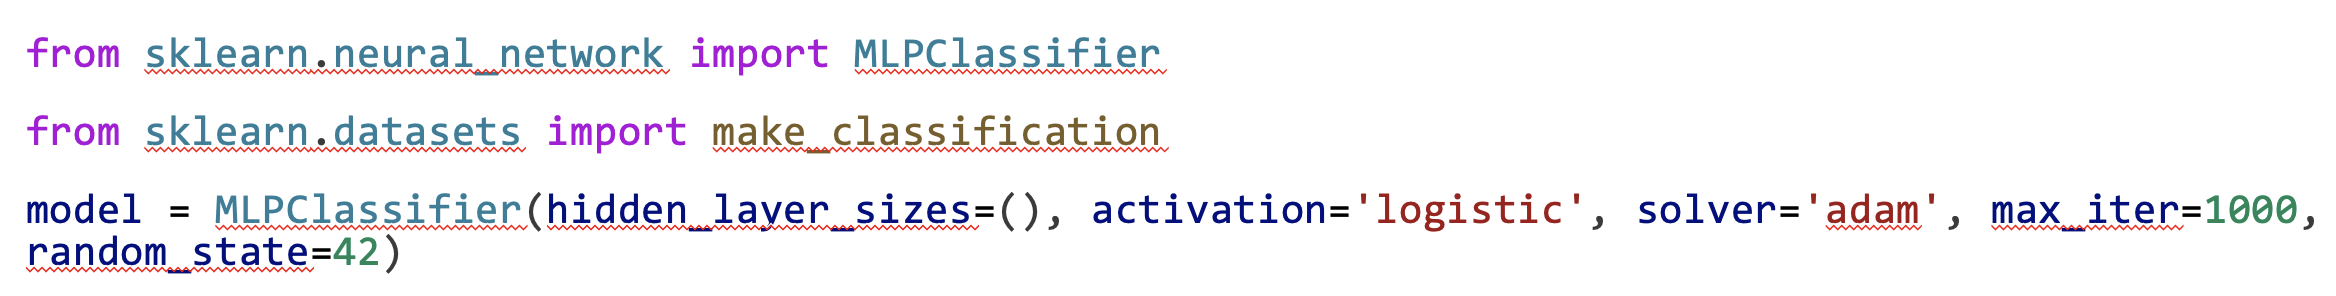
\includegraphics[width=1\linewidth]{mlp/new_codes.png}
    \caption{Import Libraries for MLP}
    \label{fig:mlp_add_code}
\end{figure}
\begin{figure}[H]
    \centering
    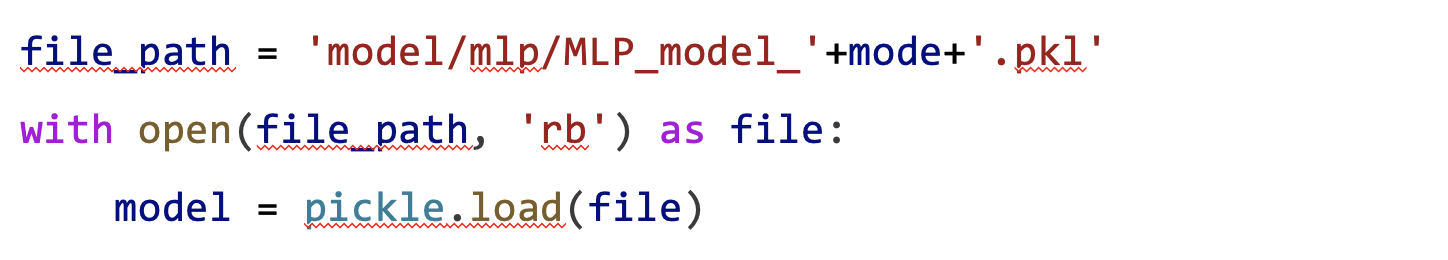
\includegraphics[width=1\linewidth]{mlp/mlpsave.png}
    \caption{Save MLP model}
    \label{fig:mlp_sve_code}
\end{figure}
\begin{figure}[H]
    \centering
    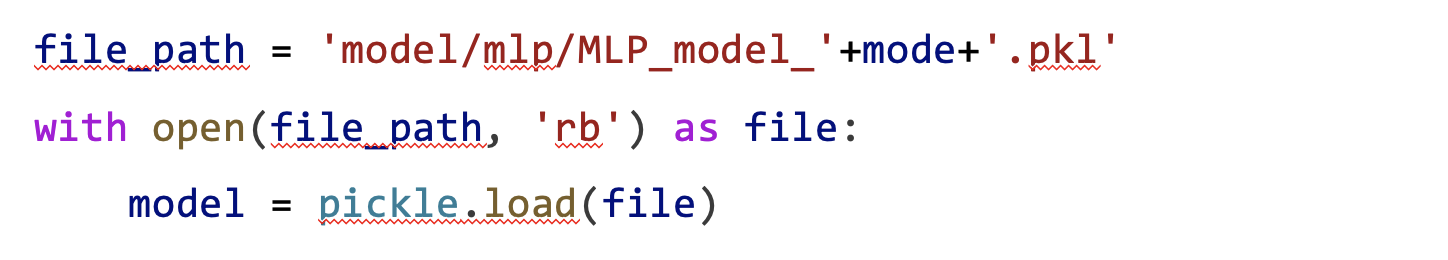
\includegraphics[width=1\linewidth]{mlp/mlpLoad.png}
    \caption{Load the MLP model}
    \label{fig:mlp_loading}
\end{figure}
\subsection{GRU}
To implement the GRU model we brought the changes added some features in the utils script and made a model file. The sample of our codes are shown in figure \ref{fig:gruheader}, \ref{fig:gruRequired}.
\begin{figure}[H]
    \centering
    
\includegraphics[width=1\linewidth]{gru/gruheader.png}
    \caption{Import Libraries for GRU}
    \label{fig:gruheader}
\end{figure}
\begin{figure}[H]
    \centering
    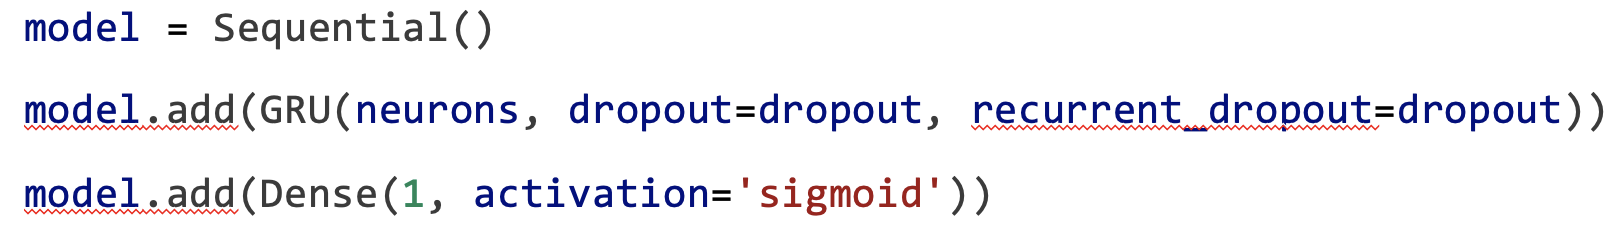
\includegraphics[width=1\linewidth]{gru/gruextra.png}
    \caption{GRU required code}
    \label{fig:gruRequired}
\end{figure}

Note: Due to the limitation in the number of pages we are not able to mention all details. We can share our overall Implementation through a repository